\section{Integralrechnung \formelbuch{483}}
\subsection{Integrationsmethoden \formelbuch{486ff}}
  
  
  \begin{tabular}{ll}
    Linearit\"at & $\int{f(\alpha x+\beta )dx=\frac{1}{\alpha}\cdot F(\alpha x+\beta)+C}$ \\
    Partielle Integration & $\int\limits_a^b{u'(x)\cdot v(x)dx}=\biggl[
    u(x)\cdot v(x) \biggr]_a^b-\int\limits_a^b{u(x)\cdot v'(x)dx}$\\
    Substitution (Rationalisierung) & $t=\tan\frac{x}{2}, \qquad
    dx=\frac{2dt}{1+t^2} \qquad \sin  x=\frac{2t}{1+t^2} \qquad \cos x=\frac{1-t^2}{1+t^2}
    \quad\int{R(\sin(x)\cos(x))dx}$\\
    Allgemeine Substitution &
    $\int\limits_{a}^{b}{f(x)dx}=\int\limits_{g^{-1}(a)}^{g^{-1}(b)}{f(g(t))\cdot
    g'(t)dt}\qquad t=g^{-1}(x)\qquad  \fbox{x=g(t)}\qquad dx=g'(t)\cdot dt$\\
    Logarithmische Integration & $\int{\frac{f'(x)}{f(x)}dx}=\ln|f(x)|+C 
    \qquad{(f(x)\neq 1)}$\\
    Spezielle Form des Integranden & $\int{f'(x)\cdot (f(x))^{\alpha} dx}=
    f(x)^{\alpha +1}\cdot \frac{1}{\alpha+1}+C
    \qquad{(\alpha \neq -1)}$\\
    Differentiation & $\int \limits ^{b} _{a} {f'(t)dt}=f(b)-f(a)$\\
    & $\frac{d}{dx} \int \limits ^{x} _{1} {f(t)dt}=f(x)$
  \end{tabular}
  
  

\subsubsection{Einige unbestimmte Integrale \formelbuch{1074 ff}}
\begin{enumerate}
  \item $ \int dx=x+C $
  \item $ \int{x^\alpha}dx=\frac{x^{\alpha+1}}{\alpha+1}+C,\ x \epsilon \mathbb
  R ^+,\ \alpha \epsilon \mathbb R \backslash \{ -1 \} $
  \item $ \int{\frac{1}{x}}dx=\ln \left| x \right| + C,\ x\neq0 $
  \item $ \int{e^x}dx=e^x+C $
  \item $ \int{a^x}dx=\frac{a^x}{\ln{a}}+C,\ a \epsilon \mathbb
  R^+\backslash\{1\} $
  \item $ \int{ \sin{x}} dx = -\cos{x} + C $
  \item $ \int{\cos{x}} dx = \sin{x} + C $
  \item $ \int{\frac{dx}{\sin^2x}}=-\cot{x}+C,\ x\neq k\pi\ \mathrm{mit}\ k
  \epsilon \mathbb Z $
  \item $ \int{\frac{dx}{\cos^2x}}=\tan{x}+C,\ x\neq\frac{\pi}{2}+k\pi\
  \mathrm{mit} k \epsilon \mathbb Z $
  %10. :
  \item $ \int{\sinh{x}}dx = \cosh{x}+C $
  \item $ \int{\cosh{x}}dx = \sinh{x}+C $
  \item $ \int{\frac{dx}{\sinh^2x}}=-\coth{x}+C,\ x\neq0 $
  \item $ \int{\frac{dx}{\cosh^2x}}=\tanh{x}+C $
  \item $ \int{\frac{dx}{ax+b}} = \frac{1}{a}\ln \left|ax + b\right| + C,\
  a\neq 0,x\neq-\frac{b}{a} $
  \item $ \int{\frac{dx}{a^2x^2+b^2}}=\frac{1}{ab}\arctan{\frac{a}{b}x}+C,\
  a\neq0,\ b\neq0 $
  \item $
  \int{\frac{dx}{a^2x^2-b^2}}=\frac{1}{2ab}\ln{\left|\frac{ax-b}{ax+b}\right|}+C,\ a\neq0,\ b\neq0,\ x\neq\frac{b}{a},\ x\neq-\frac{b}{a} $
  \item $
  \int{\sqrt{a^2x^2+b^2}}dx=\frac{x}{2}\sqrt{a^2x^2+b^2}+\frac{b^2}{2a}\ln{(ax+\sqrt{a^2x^2+b^2})}+C,\
  a\neq0,\ b\neq0 $
  \item $
  \int{\sqrt{a^2x^2-b^2}}dx=\frac{x}{2}\sqrt{a^2x^2-b^2}-\frac{b^2}{2a}\ln\left|ax+\sqrt{a^2x^2-b^2}\right|+C,\
  a\neq0,\ b\neq0,a^2x^2\geqq b^2$
  \item $
  \int\sqrt{b^2-a^2x^2}dx=\frac{x}{2}\sqrt{b^2-a^2x^2}+\frac{b^2}{2a}\arcsin\frac{a}{b}x+C,\
  a\neq0,\ b\neq0,\ a^2x^2\leqq b^2 $
  %20.:
  \item $
  \int\frac{dx}{\sqrt{a^2x^2-b^2}}=\frac{1}{a}\ln(ax+\sqrt{a^2x^2+b^2})+C,\
  a\neq0,\ b\neq0 $
  \item $
  \int\frac{dx}{\sqrt{a^2x^2-b^2}}=\frac{1}{a}\ln\left|ax+\sqrt{a^2x^2-b^2}\right|+C,\
  a\neq0,\ b\neq0,\ a^2x^2>b^2 $
  \item $ \int\frac{dx}{\sqrt{b^2-a^2x^2}}=\frac{1}{a}\arcsin\frac{a}{b}x+C,\
  a\neq0,\ b\neq0,\ a^2x^2<b^2 $
  \item Die Integrale $\int\frac{dx}{X}, \int\sqrt{X}dx,
  \int\frac{dx}{\sqrt{X}}$ mit $X=ax^2+2bx+c,\ a\neq0 $ werden durch die
  Umformung $X=a(x+\frac{b}{a})^2+(c-\frac{b^2}{a}) $ und die Substitution $
  t=x+\frac{b}{a} $ in die Integrale 15. bis 22. transformiert.
  \item $
  \int\frac{xdx}{X}=\frac{1}{2a}\ln\left|X\right|-\frac{b}{a}\int\frac{dx}{X},\ a\neq0,\ X=ax^2+2bx+c$
  \item $ \int\sin^2axdx=\frac{x}{2}-\frac{1}{4a}\cdot\sin2ax+C,\ a\neq0 $
  \item $ \int\cos^2axdx=\frac{x}{2}+\frac{1}{4a}\cdot\sin2ax+C,\ a\neq0 $
  \item $ \int\sin^naxdx=-\frac{sin^{n-1}ax\cdot\cos
  ax}{na}+\frac{n-1}{n}\int\sin^{n-2}axdx,\ n \epsilon \mathbb N,\ a\neq0 $
  \item $ \int\cos^naxdx=\frac{\cos^{n-1}ax\cdot\sin
  ax}{na}+\frac{n-1}{n}\int\cos^{n-2}axdx,\ n\epsilon \mathbb N,\ a\neq0 $
  \item $ \int\frac{dx}{\sin ax} =
  \frac{1}{a}\ln\left|\tan\frac{ax}{2}\right|+C,\ a\neq0,\ x\neq
  k\frac{\pi}{a}\ \mathrm{mit}\ k\epsilon\mathbb Z$
  %30.:
  \item $ \int\frac{dx}{\cos
  ax}=\frac{1}{a}\ln\left|\tan(\frac{ax}{2}+\frac{\pi}{4})\right|+C,\ a\neq0,\
  x\neq\frac{\pi}{2a}+k\frac{\pi}{a}\ \mathrm{mit}\ k\epsilon\mathbb Z $
  \item $\int\tan axdx=-\frac{1}{a}\ln\left|\cos ax\right|+C,\ a\neq0,\
  x\neq\frac{\pi}{2a}+k\frac{\pi}{a} \mathrm{mit}\ k\epsilon\mathbb Z$
  \item $\int\cot axdx=\frac{1}{a}\ln\left|\sin ax\right|+C,\ a\neq0,\ x\neq
  k\frac{\pi}{a} \mathrm{mit} k\epsilon\mathbb Z $
  \item $ \int x^n\sin axdx=-\frac{x^n}{a}\cos ax+\frac{n}{a}\int x^{n-1}\cos
  axdx,\ n\epsilon\mathbb N,\ a\neq0 $
  \item $ \int x^n\cos axdx=\frac{x^n}{a}\sin ax-\frac{n}{a}\int x^{n-1}\sin axdx,\ n\epsilon\mathbb N,\ a\neq0 $
  \item $ \int x^ne^{ax}dx=\frac{1}{a}x^ne^{ax}-\frac{n}{a}\int
  x^{n-1}e^{ax}dx,\ n\epsilon\mathbb N,\ a\neq0 $
  \item $ \int e^{ax}\sin bxdx=\frac{e^{ax}}{a^2+b^2}(a\sin bx-b\cos bx)+C,\
  a\neq0,\ b\neq0 $
  \item $ \int e^{ax}\cos bxdx=\frac{e^{ax}}{a^2+b^2}(a\cos bx + b\sin bx)+C,\
  a\neq0,\ b\neq0 $
  \item $ \int\ln x dx = x(\ln x-1)+C,\ x\epsilon\mathbb R^+ $
  \item $ \int x^\alpha \cdot \ln xdx =
  \frac{x^{\alpha+1}}{(\alpha+1)^2}\lbrack(\alpha+1)\ln x-1\rbrack + C,\
  x\epsilon\mathbb R^+,\ \alpha\epsilon\mathbb R\backslash\{-1\} $
  %FF1 Seite 496
\end{enumerate}

  Uneigentliches Integral heisst, dass entweder eine \textbf{unbeschr\"ankte
  Funktion} integriert wird, oder eine Funktion \"uber einen
  \textbf{unbeschr\"ankten Integrationsberech} integriert wird.$\\$
  \begin{minipage}{100mm}
    
  Für unbeschränkte Funktionen:$\\$
  $I =\int\limits _{a}^{c}f(x)dx=
  \lim\limits_{t\to 
  b-}\int\limits_{a}^{t}f(x)dx+\lim\limits_{t\to b+}\int\limits_{t}^{c}f(x)dx\\
  \\$ Für die unbeschränkte Integration:$\\$
  $I =\int\limits _{a} ^{\infty} f(x)dx= \lim \limits_{t\to \infty}\int \limits
  _{a} ^{t}f(x)dx;\\$
  $I =\int\limits ^{a} _{-\infty} f(x)dx= \lim \limits_{t\to -\infty}\int
  \limits _{t} ^{a}f(x)dx; \\$
  $I =\int\limits _{-\infty} ^{\infty} f(x)dx = \lim \limits_{t_1\to \infty} \lim
  \limits
  _{t_2 \to  \infty}\int \limits _{t_1} ^{a}f(x)dx + \int\limits_{a}^{t_2}f(x)dx\\$
  Beispiel: $\int\limits_{1}^{\infty}\frac{1}{x^2}dx=\lim\limits_{t\to \infty}\int\limits_{1}^{t}\frac{1}{x^2}dx=\lim\limits_{t\to \infty}-\frac{1}{t}+\frac{1}{1}=1$
    \end{minipage}
  \begin{minipage}{100mm}
      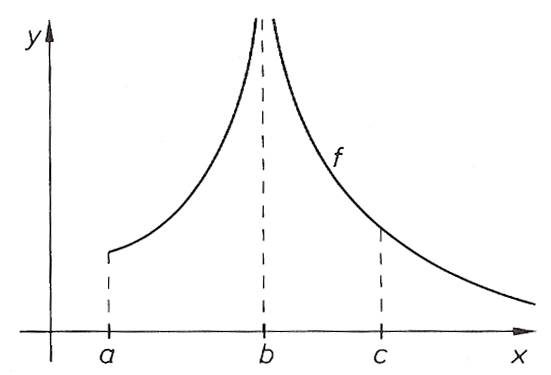
\includegraphics[width=3cm]{./bilder/unbeschraenkteFunktion.png} $\\$
      unbeschränkte Funktion
    \end{minipage}
\subsubsection{Prinzip der Restfläche}
  Wenn $\lim\limits_{t \rightarrow \infty} \int\limits^{\infty}_{t} f(x) dx = 0$, dann konvergiert
  $\int\limits_a^{\infty} f(x) dx$ und umgekehrt.

\subsubsection{Majorantenprinzip (konvergent)}
  Um nachzuweisen, ob eine Funktion $|f(x)| \geq 0$ konvergiert, wird eine zweite
  Funktion $g(x) \geq |f(x)|$ (Majorante) gesucht. Konvergiert $\int\limits_a^{\infty} g(x) dx$,
  dann konvergiert auch $\int\limits_a^{\infty} f(x) dx$. ($x \in [a, \infty)$)

\subsubsection{Minorantenprinzip (divergent)}
  Um nachzuweisen, ob eine Funktion $f(x)$ divergiert, wird eine zweite
  Funktion $0 \leq g(x) \leq f(x)$ (Minorante) gesucht. Divergiert
  $\int\limits_a^{\infty} g(x) dx$,
  dann divergiert auch $\int\limits_a^{\infty} f(x) dx$. ($x \in [a, \infty)$)
  